\documentclass{book}
\usepackage[a4paper,top=2.5cm,bottom=2.5cm,left=2.5cm,right=2.5cm]{geometry}
\usepackage{makeidx}
\usepackage{natbib}
\usepackage{graphicx}
\usepackage{multicol}
\usepackage{float}
\usepackage{listings}
\usepackage{color}
\usepackage{ifthen}
\usepackage[table]{xcolor}
\usepackage{textcomp}
\usepackage{alltt}
\usepackage{ifpdf}
\ifpdf
\usepackage[pdftex,
            pagebackref=true,
            colorlinks=true,
            linkcolor=blue,
            unicode
           ]{hyperref}
\else
\usepackage[ps2pdf,
            pagebackref=true,
            colorlinks=true,
            linkcolor=blue,
            unicode
           ]{hyperref}
\usepackage{pspicture}
\fi
\usepackage[utf8]{inputenc}
\usepackage{mathptmx}
\usepackage[scaled=.90]{helvet}
\usepackage{courier}
\usepackage{sectsty}
\usepackage{amssymb}
\usepackage[titles]{tocloft}
\usepackage{doxygen}
\lstset{language=C++,inputencoding=utf8,basicstyle=\footnotesize,breaklines=true,breakatwhitespace=true,tabsize=4,numbers=left }
\makeindex
\setcounter{tocdepth}{3}
\renewcommand{\footrulewidth}{0.4pt}
\renewcommand{\familydefault}{\sfdefault}
\hfuzz=15pt
\setlength{\emergencystretch}{15pt}
\hbadness=750
\tolerance=750
\begin{document}
\hypersetup{pageanchor=false,citecolor=blue}
\begin{titlepage}
\vspace*{7cm}
\begin{center}
{\Large A\-E\-D\-A T\-P1 2013/2014 }\\
\vspace*{1cm}
{\large Generated by Doxygen 1.8.3}\\
\vspace*{0.5cm}
{\small Mon Nov 11 2013 23:24:37}\\
\end{center}
\end{titlepage}
\clearemptydoublepage
\pagenumbering{roman}
\tableofcontents
\clearemptydoublepage
\pagenumbering{arabic}
\hypersetup{pageanchor=true,citecolor=blue}
\chapter{Hierarchical Index}
\section{Class Hierarchy}
This inheritance list is sorted roughly, but not completely, alphabetically\-:\begin{DoxyCompactList}
\item \contentsline{section}{Aluno\-Nao\-Existente}{\pageref{class_aluno_nao_existente}}{}
\item \contentsline{section}{Alunos\-Por\-Turma\-Excedido}{\pageref{class_alunos_por_turma_excedido}}{}
\item \contentsline{section}{Disciplina}{\pageref{class_disciplina}}{}
\item \contentsline{section}{Disciplina\-Nao\-Existente}{\pageref{class_disciplina_nao_existente}}{}
\item \contentsline{section}{Duracao\-Excedida}{\pageref{class_duracao_excedida}}{}
\item \contentsline{section}{Escola}{\pageref{class_escola}}{}
\item \contentsline{section}{Horario}{\pageref{class_horario}}{}
\item \contentsline{section}{Pessoa}{\pageref{class_pessoa}}{}
\begin{DoxyCompactList}
\item \contentsline{section}{Aluno}{\pageref{class_aluno}}{}
\item \contentsline{section}{Professor}{\pageref{class_professor}}{}
\begin{DoxyCompactList}
\item \contentsline{section}{Director\-Turma}{\pageref{class_director_turma}}{}
\end{DoxyCompactList}
\end{DoxyCompactList}
\item \contentsline{section}{Professor\-Nao\-Existente}{\pageref{class_professor_nao_existente}}{}
\item \contentsline{section}{Turma}{\pageref{class_turma}}{}
\item \contentsline{section}{Turma\-Existente}{\pageref{class_turma_existente}}{}
\item \contentsline{section}{Turma\-Nao\-Existente}{\pageref{class_turma_nao_existente}}{}
\end{DoxyCompactList}

\chapter{Class Index}
\section{Class List}
Here are the classes, structs, unions and interfaces with brief descriptions\-:\begin{DoxyCompactList}
\item\contentsline{section}{\hyperlink{class_aluno}{Aluno} \\*\hyperlink{class_aluno}{Aluno} de uma escola }{\pageref{class_aluno}}{}
\item\contentsline{section}{\hyperlink{class_aluno_nao_existente}{Aluno\-Nao\-Existente} \\*Excepcao lancada quando o \hyperlink{class_aluno}{Aluno} a ser acedido nao existe }{\pageref{class_aluno_nao_existente}}{}
\item\contentsline{section}{\hyperlink{class_alunos_por_turma_excedido}{Alunos\-Por\-Turma\-Excedido} \\*Excep�ao lancada quando o numero de alunos por turma � excedido }{\pageref{class_alunos_por_turma_excedido}}{}
\item\contentsline{section}{\hyperlink{class_director_turma}{Director\-Turma} \\*Classe derivado de \hyperlink{class_professor}{Professor} tendo a mais um vector com as turmas de que e responsavel }{\pageref{class_director_turma}}{}
\item\contentsline{section}{\hyperlink{class_disciplina}{Disciplina} \\*Class representa uma \hyperlink{class_disciplina}{Disciplina} contendo a sua designacao, duracao e hora de inicio }{\pageref{class_disciplina}}{}
\item\contentsline{section}{\hyperlink{class_disciplina_nao_existente}{Disciplina\-Nao\-Existente} \\*Excepcao lancada quando o \hyperlink{class_professor}{Professor} a ser acedido nao existe }{\pageref{class_disciplina_nao_existente}}{}
\item\contentsline{section}{\hyperlink{class_duracao_excedida}{Duracao\-Excedida} }{\pageref{class_duracao_excedida}}{}
\item\contentsline{section}{\hyperlink{class_escola}{Escola} \\*Representa uma \hyperlink{class_escola}{Escola} contendo todos os seus Alunos, Professores, Turmas, Disciplinas e Horarios }{\pageref{class_escola}}{}
\item\contentsline{section}{\hyperlink{class_horario}{Horario} \\*Hor�rio de uma \hyperlink{class_turma}{Turma} }{\pageref{class_horario}}{}
\item\contentsline{section}{\hyperlink{class_pessoa}{Pessoa} \\*Classe Base para \hyperlink{class_professor}{Professor} e \hyperlink{class_aluno}{Aluno} }{\pageref{class_pessoa}}{}
\item\contentsline{section}{\hyperlink{class_professor}{Professor} \\*\hyperlink{class_professor}{Professor} de uma \hyperlink{class_escola}{Escola} (class Base), podendo ou nao ser Director de \hyperlink{class_turma}{Turma} }{\pageref{class_professor}}{}
\item\contentsline{section}{\hyperlink{class_professor_nao_existente}{Professor\-Nao\-Existente} \\*Excepcao lancada quando o \hyperlink{class_professor}{Professor} a ser acedido nao existe }{\pageref{class_professor_nao_existente}}{}
\item\contentsline{section}{\hyperlink{class_turma}{Turma} }{\pageref{class_turma}}{}
\item\contentsline{section}{\hyperlink{class_turma_existente}{Turma\-Existente} \\*Excepcao lancada quando uma \hyperlink{class_turma}{Turma} a ser adicionada ao vector de Turmas de uma \hyperlink{class_professor}{Professor} que ja contem a mesma }{\pageref{class_turma_existente}}{}
\item\contentsline{section}{\hyperlink{class_turma_nao_existente}{Turma\-Nao\-Existente} \\*Excepcao lancada quando a \hyperlink{class_turma}{Turma} a ser acedida nao existe }{\pageref{class_turma_nao_existente}}{}
\end{DoxyCompactList}

\chapter{Class Documentation}
\hypertarget{class_aluno}{\section{Aluno Class Reference}
\label{class_aluno}\index{Aluno@{Aluno}}
}
\subsection*{Public Member Functions}
\begin{DoxyCompactItemize}
\item 
\hypertarget{class_aluno_ade694c179acf4d2c82abec8ee44d1793}{{\bfseries Aluno} (string nome, int numero, \hyperlink{class_turma}{Turma} $\ast$t)}\label{class_aluno_ade694c179acf4d2c82abec8ee44d1793}

\item 
\hypertarget{class_aluno_a75ca576e335d4678e6777de92a218b99}{string {\bfseries get\-Nome} ()}\label{class_aluno_a75ca576e335d4678e6777de92a218b99}

\item 
\hypertarget{class_aluno_a258e8f5c3dbc8b19efadaf20ba48874f}{int {\bfseries get\-Numero} ()}\label{class_aluno_a258e8f5c3dbc8b19efadaf20ba48874f}

\item 
\hypertarget{class_aluno_a1f3d823c2589d39d930738689707ba3d}{\hyperlink{class_turma}{Turma} $\ast$ {\bfseries get\-Turma} ()}\label{class_aluno_a1f3d823c2589d39d930738689707ba3d}

\item 
\hypertarget{class_aluno_a317539f87c1d2cd5d0228eef9b42bd14}{void {\bfseries set\-Nome} (string nome)}\label{class_aluno_a317539f87c1d2cd5d0228eef9b42bd14}

\item 
\hypertarget{class_aluno_a36ad83483a9e0c247d7092a95607758c}{void {\bfseries set\-Numero} (int numero)}\label{class_aluno_a36ad83483a9e0c247d7092a95607758c}

\item 
\hypertarget{class_aluno_a5403cd3d2d1a219f9aa49bc53825d4fc}{void {\bfseries set\-Turma} (\hyperlink{class_turma}{Turma} $\ast$t)}\label{class_aluno_a5403cd3d2d1a219f9aa49bc53825d4fc}

\item 
\hypertarget{class_aluno_a70c5a814dcd56edc12bbe2c00aa3a7a6}{bool {\bfseries operator==} (\hyperlink{class_aluno}{Aluno} $\ast$a2)}\label{class_aluno_a70c5a814dcd56edc12bbe2c00aa3a7a6}

\end{DoxyCompactItemize}


The documentation for this class was generated from the following files\-:\begin{DoxyCompactItemize}
\item 
Aluno.\-h\item 
Aluno.\-cpp\end{DoxyCompactItemize}

\hypertarget{class_aluno_nao_existente}{\section{Aluno\-Nao\-Existente Class Reference}
\label{class_aluno_nao_existente}\index{Aluno\-Nao\-Existente@{Aluno\-Nao\-Existente}}
}


Excepcao lancada quando o \hyperlink{class_aluno}{Aluno} a ser acedido nao existe.  




{\ttfamily \#include $<$Excepcao.\-h$>$}

\subsection*{Public Member Functions}
\begin{DoxyCompactItemize}
\item 
\hypertarget{class_aluno_nao_existente_a5ad5fa0f402f1bec2b88b698cf3f5928}{{\bfseries Aluno\-Nao\-Existente} (\hyperlink{class_aluno}{Aluno} $\ast$a)}\label{class_aluno_nao_existente_a5ad5fa0f402f1bec2b88b698cf3f5928}

\item 
string \hyperlink{class_aluno_nao_existente_aacfbce6e5c3fba7f14cdfe4588d9f3fc}{get\-Erro} ()
\item 
\hypertarget{class_aluno_nao_existente_a72857c8ba816dbec308567382904e14b}{virtual \hyperlink{class_aluno_nao_existente_a72857c8ba816dbec308567382904e14b}{$\sim$\-Aluno\-Nao\-Existente} ()}\label{class_aluno_nao_existente_a72857c8ba816dbec308567382904e14b}

\begin{DoxyCompactList}\small\item\em Destrutor. \end{DoxyCompactList}\end{DoxyCompactItemize}
\subsection*{Public Attributes}
\begin{DoxyCompactItemize}
\item 
\hypertarget{class_aluno_nao_existente_a094d853c6593f3b82363171adbcd2158}{\hyperlink{class_aluno}{Aluno} $\ast$ \hyperlink{class_aluno_nao_existente_a094d853c6593f3b82363171adbcd2158}{aluno}}\label{class_aluno_nao_existente_a094d853c6593f3b82363171adbcd2158}

\begin{DoxyCompactList}\small\item\em \hyperlink{class_aluno}{Aluno} inesxistente. \end{DoxyCompactList}\end{DoxyCompactItemize}


\subsection{Detailed Description}
Excepcao lancada quando o \hyperlink{class_aluno}{Aluno} a ser acedido nao existe. 

\subsection{Member Function Documentation}
\hypertarget{class_aluno_nao_existente_aacfbce6e5c3fba7f14cdfe4588d9f3fc}{\index{Aluno\-Nao\-Existente@{Aluno\-Nao\-Existente}!get\-Erro@{get\-Erro}}
\index{get\-Erro@{get\-Erro}!AlunoNaoExistente@{Aluno\-Nao\-Existente}}
\subsubsection[{get\-Erro}]{\setlength{\rightskip}{0pt plus 5cm}string Aluno\-Nao\-Existente\-::get\-Erro (
\begin{DoxyParamCaption}
{}
\end{DoxyParamCaption}
)\hspace{0.3cm}{\ttfamily [inline]}}}\label{class_aluno_nao_existente_aacfbce6e5c3fba7f14cdfe4588d9f3fc}
$<$ Mensagem de erro lancada pela excepcao 

The documentation for this class was generated from the following file\-:\begin{DoxyCompactItemize}
\item 
Excepcao.\-h\end{DoxyCompactItemize}

\hypertarget{class_alunos_por_turma_excedido}{\section{Alunos\-Por\-Turma\-Excedido Class Reference}
\label{class_alunos_por_turma_excedido}\index{Alunos\-Por\-Turma\-Excedido@{Alunos\-Por\-Turma\-Excedido}}
}


Excep�ao lancada quando o numero de alunos por turma � excedido.  




{\ttfamily \#include $<$Excepcao.\-h$>$}

\subsection*{Public Member Functions}
\begin{DoxyCompactItemize}
\item 
\hypertarget{class_alunos_por_turma_excedido_a34a212882e9b566992c4e9cf618e1425}{{\bfseries Alunos\-Por\-Turma\-Excedido} (\hyperlink{class_aluno}{Aluno} $\ast$a)}\label{class_alunos_por_turma_excedido_a34a212882e9b566992c4e9cf618e1425}

\item 
string \hyperlink{class_alunos_por_turma_excedido_a5c9495949ceaf62e87e6ee03cf596b9e}{get\-Erro} ()
\item 
\hypertarget{class_alunos_por_turma_excedido_a018e25ae5eb0bfc4f704561c9f951c11}{virtual \hyperlink{class_alunos_por_turma_excedido_a018e25ae5eb0bfc4f704561c9f951c11}{$\sim$\-Alunos\-Por\-Turma\-Excedido} ()}\label{class_alunos_por_turma_excedido_a018e25ae5eb0bfc4f704561c9f951c11}

\begin{DoxyCompactList}\small\item\em Destrutor. \end{DoxyCompactList}\end{DoxyCompactItemize}
\subsection*{Public Attributes}
\begin{DoxyCompactItemize}
\item 
\hypertarget{class_alunos_por_turma_excedido_ad3b26da7b4a81b52cd2e1cf969cbae2e}{\hyperlink{class_aluno}{Aluno} $\ast$ \hyperlink{class_alunos_por_turma_excedido_ad3b26da7b4a81b52cd2e1cf969cbae2e}{aluno}}\label{class_alunos_por_turma_excedido_ad3b26da7b4a81b52cd2e1cf969cbae2e}

\begin{DoxyCompactList}\small\item\em \hyperlink{class_aluno}{Aluno} que excede o limite da turma. \end{DoxyCompactList}\end{DoxyCompactItemize}


\subsection{Detailed Description}
Excep�ao lancada quando o numero de alunos por turma � excedido. 

\subsection{Member Function Documentation}
\hypertarget{class_alunos_por_turma_excedido_a5c9495949ceaf62e87e6ee03cf596b9e}{\index{Alunos\-Por\-Turma\-Excedido@{Alunos\-Por\-Turma\-Excedido}!get\-Erro@{get\-Erro}}
\index{get\-Erro@{get\-Erro}!AlunosPorTurmaExcedido@{Alunos\-Por\-Turma\-Excedido}}
\subsubsection[{get\-Erro}]{\setlength{\rightskip}{0pt plus 5cm}string Alunos\-Por\-Turma\-Excedido\-::get\-Erro (
\begin{DoxyParamCaption}
{}
\end{DoxyParamCaption}
)\hspace{0.3cm}{\ttfamily [inline]}}}\label{class_alunos_por_turma_excedido_a5c9495949ceaf62e87e6ee03cf596b9e}
$<$ Mensagem de erro lancada pela excepcao 

The documentation for this class was generated from the following file\-:\begin{DoxyCompactItemize}
\item 
Excepcao.\-h\end{DoxyCompactItemize}

\hypertarget{class_director_turma}{\section{Director\-Turma Class Reference}
\label{class_director_turma}\index{Director\-Turma@{Director\-Turma}}
}


Classe derivado de \hyperlink{class_professor}{Professor} tendo a mais um vector com as turmas de que e responsavel.  




{\ttfamily \#include $<$Professor.\-h$>$}

Inheritance diagram for Director\-Turma\-:\begin{figure}[H]
\begin{center}
\leavevmode
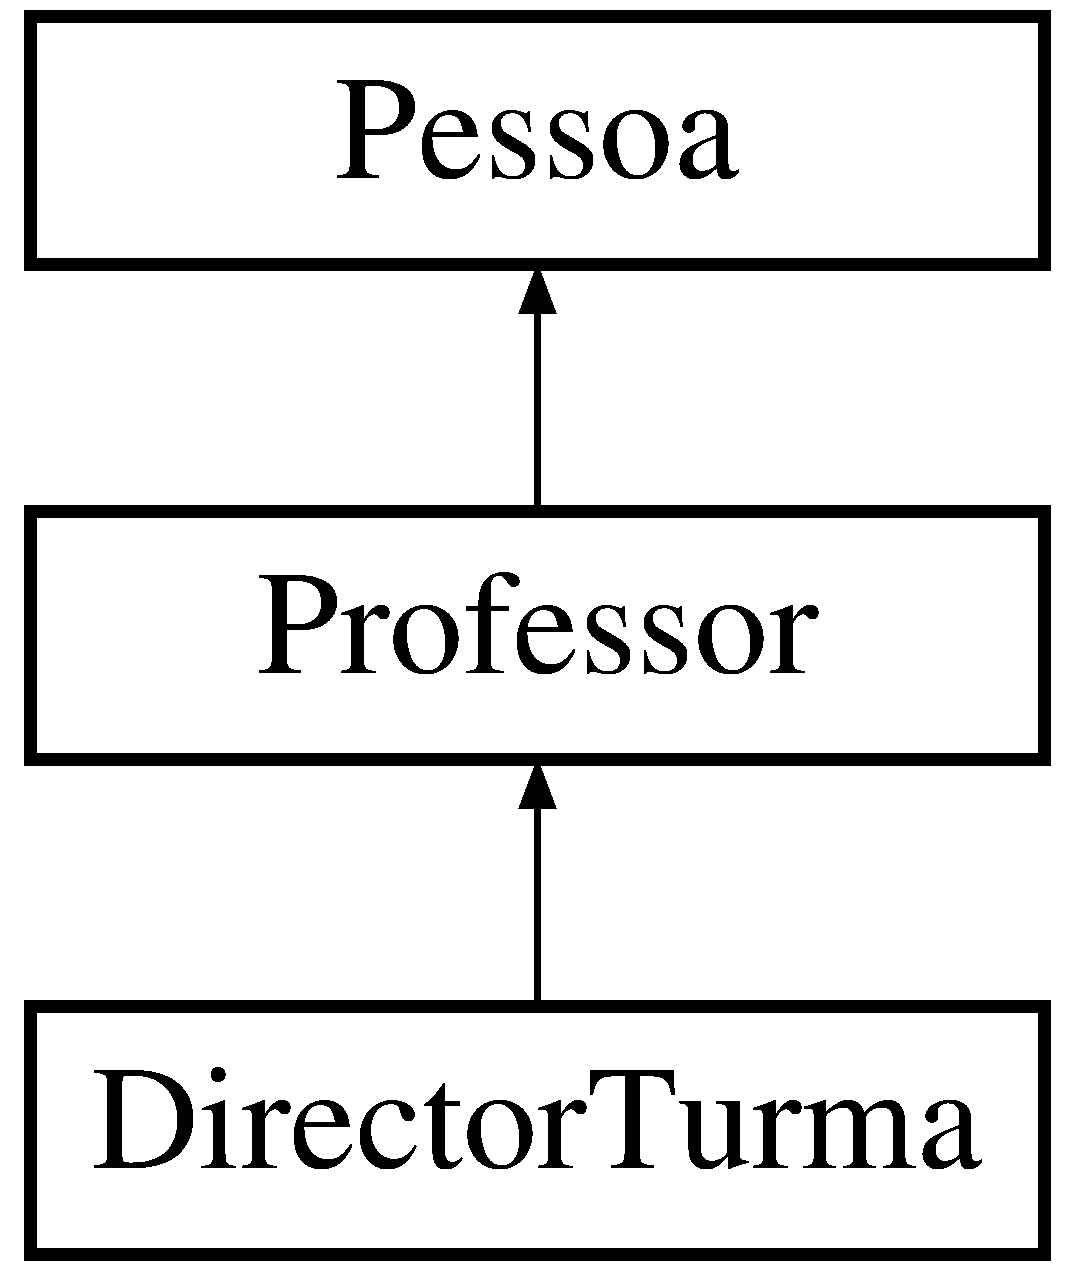
\includegraphics[height=3.000000cm]{class_director_turma}
\end{center}
\end{figure}
\subsection*{Public Member Functions}
\begin{DoxyCompactItemize}
\item 
\hypertarget{class_director_turma_a68cae9fe812395183f4da5e8b2f5cfe6}{{\bfseries Director\-Turma} (string n, \hyperlink{class_disciplina}{Disciplina} $\ast$d, \hyperlink{class_turma}{Turma} $\ast$t, \hyperlink{class_turma}{Turma} $\ast$t\-\_\-responsavel)}\label{class_director_turma_a68cae9fe812395183f4da5e8b2f5cfe6}

\item 
\hypertarget{class_director_turma_a99567238fee363836711fb01e7b49617}{bool {\bfseries add\-Turma\-Responsavel} (\hyperlink{class_turma}{Turma} $\ast$t)}\label{class_director_turma_a99567238fee363836711fb01e7b49617}

\item 
\hypertarget{class_director_turma_a08f76bfffd82b428bd601773fe44a26e}{bool {\bfseries remove\-Turma\-Responsavel} (const int id)}\label{class_director_turma_a08f76bfffd82b428bd601773fe44a26e}

\item 
\hypertarget{class_director_turma_ad481d568f5e9f30ddcfa6a6c65daaf1b}{vector$<$ \hyperlink{class_turma}{Turma} $\ast$ $>$ {\bfseries get\-Turmas\-Responsaveis} ()}\label{class_director_turma_ad481d568f5e9f30ddcfa6a6c65daaf1b}

\end{DoxyCompactItemize}


\subsection{Detailed Description}
Classe derivado de \hyperlink{class_professor}{Professor} tendo a mais um vector com as turmas de que e responsavel. 

The documentation for this class was generated from the following files\-:\begin{DoxyCompactItemize}
\item 
Professor.\-h\item 
Professor.\-cpp\end{DoxyCompactItemize}

\hypertarget{class_disciplina}{\section{Disciplina Class Reference}
\label{class_disciplina}\index{Disciplina@{Disciplina}}
}


Class representa uma \hyperlink{class_disciplina}{Disciplina} contendo a sua designacao, duracao e hora de inicio.  




{\ttfamily \#include $<$Disciplina.\-h$>$}

\subsection*{Public Member Functions}
\begin{DoxyCompactItemize}
\item 
\hypertarget{class_disciplina_ae4496d51677842852775c89892387daf}{{\bfseries Disciplina} (string \-\_\-nome, int d, int h)}\label{class_disciplina_ae4496d51677842852775c89892387daf}

\item 
\hypertarget{class_disciplina_a09445908668708d2b62feb8b600a6af6}{string {\bfseries get\-Nome} () const }\label{class_disciplina_a09445908668708d2b62feb8b600a6af6}

\item 
\hypertarget{class_disciplina_a2d8e0957375f6d9f1f720a58acfb80de}{void {\bfseries set\-Nome} (string \-\_\-nome)}\label{class_disciplina_a2d8e0957375f6d9f1f720a58acfb80de}

\item 
\hypertarget{class_disciplina_aa3f19dc881279231e7eaa3194f01c4df}{int {\bfseries get\-Duracao} () const }\label{class_disciplina_aa3f19dc881279231e7eaa3194f01c4df}

\item 
\hypertarget{class_disciplina_aadc65f8c2f09352cc6f80881d67e720d}{void {\bfseries set\-Duracao} (int d)}\label{class_disciplina_aadc65f8c2f09352cc6f80881d67e720d}

\item 
\hypertarget{class_disciplina_afde765c64f78f530d09d404d15c4c5dd}{int {\bfseries get\-Hora\-Inicio} () const }\label{class_disciplina_afde765c64f78f530d09d404d15c4c5dd}

\item 
\hypertarget{class_disciplina_aa6822138c1277be2b2c5c420c1a1f34d}{void {\bfseries set\-Hora\-Inicio} (int h)}\label{class_disciplina_aa6822138c1277be2b2c5c420c1a1f34d}

\item 
\hypertarget{class_disciplina_a28b929f7e36d902da32b0ecc329420b6}{int {\bfseries get\-Hora\-Fim} () const }\label{class_disciplina_a28b929f7e36d902da32b0ecc329420b6}

\item 
\hypertarget{class_disciplina_a41f649eceb91b6e2cae441a5888c7b84}{bool {\bfseries operator==} (\hyperlink{class_disciplina}{Disciplina} $\ast$d2)}\label{class_disciplina_a41f649eceb91b6e2cae441a5888c7b84}

\end{DoxyCompactItemize}


\subsection{Detailed Description}
Class representa uma \hyperlink{class_disciplina}{Disciplina} contendo a sua designacao, duracao e hora de inicio. 

The documentation for this class was generated from the following files\-:\begin{DoxyCompactItemize}
\item 
Disciplina.\-h\item 
Disciplina.\-cpp\end{DoxyCompactItemize}

\hypertarget{class_disciplina_nao_existente}{\section{Disciplina\-Nao\-Existente Class Reference}
\label{class_disciplina_nao_existente}\index{Disciplina\-Nao\-Existente@{Disciplina\-Nao\-Existente}}
}


Excepcao lancada quando o \hyperlink{class_professor}{Professor} a ser acedido nao existe.  




{\ttfamily \#include $<$Excepcao.\-h$>$}

\subsection*{Public Member Functions}
\begin{DoxyCompactItemize}
\item 
\hypertarget{class_disciplina_nao_existente_a6a31b19d16df94d71d2ee360600d5150}{{\bfseries Disciplina\-Nao\-Existente} (\hyperlink{class_disciplina}{Disciplina} $\ast$d)}\label{class_disciplina_nao_existente_a6a31b19d16df94d71d2ee360600d5150}

\item 
string \hyperlink{class_disciplina_nao_existente_a6a201b94440edd339ec05d1e9db8319b}{get\-Erro} ()
\item 
\hypertarget{class_disciplina_nao_existente_a4c0655a54da71a17d8f0fba702cf374d}{virtual \hyperlink{class_disciplina_nao_existente_a4c0655a54da71a17d8f0fba702cf374d}{$\sim$\-Disciplina\-Nao\-Existente} ()}\label{class_disciplina_nao_existente_a4c0655a54da71a17d8f0fba702cf374d}

\begin{DoxyCompactList}\small\item\em Destrutor. \end{DoxyCompactList}\end{DoxyCompactItemize}
\subsection*{Public Attributes}
\begin{DoxyCompactItemize}
\item 
\hypertarget{class_disciplina_nao_existente_ad681e3d7b6ba5c6120b23084bf4ae657}{\hyperlink{class_disciplina}{Disciplina} $\ast$ \hyperlink{class_disciplina_nao_existente_ad681e3d7b6ba5c6120b23084bf4ae657}{disciplina}}\label{class_disciplina_nao_existente_ad681e3d7b6ba5c6120b23084bf4ae657}

\begin{DoxyCompactList}\small\item\em \hyperlink{class_aluno}{Aluno} inesxistente. \end{DoxyCompactList}\end{DoxyCompactItemize}


\subsection{Detailed Description}
Excepcao lancada quando o \hyperlink{class_professor}{Professor} a ser acedido nao existe. 

\subsection{Member Function Documentation}
\hypertarget{class_disciplina_nao_existente_a6a201b94440edd339ec05d1e9db8319b}{\index{Disciplina\-Nao\-Existente@{Disciplina\-Nao\-Existente}!get\-Erro@{get\-Erro}}
\index{get\-Erro@{get\-Erro}!DisciplinaNaoExistente@{Disciplina\-Nao\-Existente}}
\subsubsection[{get\-Erro}]{\setlength{\rightskip}{0pt plus 5cm}string Disciplina\-Nao\-Existente\-::get\-Erro (
\begin{DoxyParamCaption}
{}
\end{DoxyParamCaption}
)\hspace{0.3cm}{\ttfamily [inline]}}}\label{class_disciplina_nao_existente_a6a201b94440edd339ec05d1e9db8319b}
$<$ Mensagem de erro lancada pela excepcao 

The documentation for this class was generated from the following file\-:\begin{DoxyCompactItemize}
\item 
Excepcao.\-h\end{DoxyCompactItemize}

\hypertarget{class_duracao_excedida}{\section{Duracao\-Excedida Class Reference}
\label{class_duracao_excedida}\index{Duracao\-Excedida@{Duracao\-Excedida}}
}
\subsection*{Public Member Functions}
\begin{DoxyCompactItemize}
\item 
\hypertarget{class_duracao_excedida_a99e2ea6501cd6c8191b36395c2216055}{{\bfseries Duracao\-Excedida} (int d)}\label{class_duracao_excedida_a99e2ea6501cd6c8191b36395c2216055}

\item 
\hypertarget{class_duracao_excedida_af83836450fa7d721d277b80e6b145ff4}{string {\bfseries get\-Erro} () const }\label{class_duracao_excedida_af83836450fa7d721d277b80e6b145ff4}

\end{DoxyCompactItemize}
\subsection*{Public Attributes}
\begin{DoxyCompactItemize}
\item 
\hypertarget{class_duracao_excedida_a9a6e5e0de552c9c6d10e8b387e7db03a}{int {\bfseries \-\_\-duracao}}\label{class_duracao_excedida_a9a6e5e0de552c9c6d10e8b387e7db03a}

\end{DoxyCompactItemize}


The documentation for this class was generated from the following file\-:\begin{DoxyCompactItemize}
\item 
Excepcao.\-h\end{DoxyCompactItemize}

\hypertarget{class_escola}{\section{Escola Class Reference}
\label{class_escola}\index{Escola@{Escola}}
}


Representa uma \hyperlink{class_escola}{Escola} contendo todos os seus Alunos, Professores, Turmas, Disciplinas e Horarios.  




{\ttfamily \#include $<$Escola.\-h$>$}

\subsection*{Public Member Functions}
\begin{DoxyCompactItemize}
\item 
vector$<$ \hyperlink{class_aluno}{Aluno} $\ast$ $>$ \hyperlink{class_escola_a881727d5171216be19d3e63cf95e2110}{get\-Alunos} ()
\item 
\hypertarget{class_escola_a56f72e713a433a9b63086df24de6985a}{void \hyperlink{class_escola_a56f72e713a433a9b63086df24de6985a}{set\-Aluno} (\hyperlink{class_aluno}{Aluno} $\ast$a)}\label{class_escola_a56f72e713a433a9b63086df24de6985a}

\begin{DoxyCompactList}\small\item\em Acrescenta alunos ao vector \-\_\-alunos. \end{DoxyCompactList}\item 
\hyperlink{class_aluno}{Aluno} $\ast$ \hyperlink{class_escola_a7582a678219ca0977bab1ac1db1109f2}{get\-Aluno\-By\-Nome} (string n)
\begin{DoxyCompactList}\small\item\em Devolve o \hyperlink{class_aluno}{Aluno} com o nome igual a n. \end{DoxyCompactList}\item 
bool \hyperlink{class_escola_ab8911a8daa03ac6172defbcb68710b06}{add\-Aluno} (string nome, int numero, \hyperlink{class_turma}{Turma} $\ast$t)
\begin{DoxyCompactList}\small\item\em Adiciona um \hyperlink{class_aluno}{Aluno} a \hyperlink{class_escola}{Escola}. \end{DoxyCompactList}\item 
string \hyperlink{class_escola_a61476572624adfbc5ff2a0dce1e8ce0b}{show\-Aluno} (\hyperlink{class_aluno}{Aluno} $\ast$a)
\begin{DoxyCompactList}\small\item\em Mostra o \hyperlink{class_aluno}{Aluno} no ecra. \end{DoxyCompactList}\item 
bool \hyperlink{class_escola_ab8ae7317b753dbe8308a60ac39d4f714}{update\-Aluno} (\hyperlink{class_aluno}{Aluno} $\ast$a)
\begin{DoxyCompactList}\small\item\em Altera informacao do \hyperlink{class_aluno}{Aluno}. \end{DoxyCompactList}\item 
bool \hyperlink{class_escola_acfa55addf5866a486acdfdc84ee9c66a}{remove\-Aluno} (\hyperlink{class_aluno}{Aluno} $\ast$a)
\begin{DoxyCompactList}\small\item\em Remove um \hyperlink{class_aluno}{Aluno} da \hyperlink{class_escola}{Escola}. \end{DoxyCompactList}\item 
vector$<$ \hyperlink{class_professor}{Professor} $\ast$ $>$ \hyperlink{class_escola_a8cdb86f03082f15f5f3ce63d1ae0b1f2}{get\-Professores} ()
\begin{DoxyCompactList}\small\item\em Devolve todos os professores existentes na \hyperlink{class_escola}{Escola}. \end{DoxyCompactList}\item 
void \hyperlink{class_escola_a69bc6d8eb743a508d2b805285fd59e35}{set\-Professor} (\hyperlink{class_professor}{Professor} $\ast$p)
\begin{DoxyCompactList}\small\item\em Acrescenta professores ao vector \-\_\-professores. \end{DoxyCompactList}\item 
\hyperlink{class_professor}{Professor} $\ast$ \hyperlink{class_escola_a1f0dba75b82a3aec3cdaccafec4350c3}{get\-Professor\-By\-Nome} (const string n)
\begin{DoxyCompactList}\small\item\em Devolve o \hyperlink{class_professor}{Professor} com o nome igual a n. \end{DoxyCompactList}\item 
bool \hyperlink{class_escola_a9cb288aece2339850bd18eaf1614f8b9}{add\-Professor} (string n, string d, int t)
\begin{DoxyCompactList}\small\item\em Adiciona um \hyperlink{class_professor}{Professor} a \hyperlink{class_escola}{Escola}. \end{DoxyCompactList}\item 
string \hyperlink{class_escola_addc6cd7b85c6fdba76dd536c580c16c8}{show\-Professor} (\hyperlink{class_professor}{Professor} $\ast$p)
\begin{DoxyCompactList}\small\item\em Mostra o \hyperlink{class_professor}{Professor} no ecra. \end{DoxyCompactList}\item 
bool \hyperlink{class_escola_a409612d09d981eb7e6e3a532080d7aed}{update\-Professor} (\hyperlink{class_professor}{Professor} $\ast$p)
\begin{DoxyCompactList}\small\item\em Altera a informacao do \hyperlink{class_professor}{Professor}. \end{DoxyCompactList}\item 
bool \hyperlink{class_escola_ab88ff73f646f14380fdbb5a55bc49882}{remove\-Professor} (const string n)
\begin{DoxyCompactList}\small\item\em Remove um \hyperlink{class_professor}{Professor} da \hyperlink{class_escola}{Escola}. \end{DoxyCompactList}\item 
vector$<$ \hyperlink{class_turma}{Turma} $\ast$ $>$ \hyperlink{class_escola_acee757e16892f33820b22a7d7749d97d}{get\-Turmas} ()
\begin{DoxyCompactList}\small\item\em Devolve todas as turmas existentes na \hyperlink{class_escola}{Escola}. \end{DoxyCompactList}\item 
void \hyperlink{class_escola_a75635f871c420f3d1373285b1e773ce8}{set\-Turma} (\hyperlink{class_turma}{Turma} $\ast$t)
\begin{DoxyCompactList}\small\item\em Acrescenta turmas ao vector turmas. \end{DoxyCompactList}\item 
\hyperlink{class_turma}{Turma} $\ast$ \hyperlink{class_escola_a5dab98b3f36b81a764b104d9d9a302e8}{get\-Turma\-By\-Id} (int id)
\begin{DoxyCompactList}\small\item\em Devolve a \hyperlink{class_turma}{Turma} com o id igual a id. \end{DoxyCompactList}\item 
bool \hyperlink{class_escola_a86d547f74fe935bfd8bdf3cd35d25860}{add\-Turma} (int id, int ano\-Escolar)
\begin{DoxyCompactList}\small\item\em Adiciona uma \hyperlink{class_turma}{Turma} a \hyperlink{class_escola}{Escola}. \end{DoxyCompactList}\item 
string \hyperlink{class_escola_a91096932c5326cb2e5c30cbd860c126c}{show\-Turma} (\hyperlink{class_turma}{Turma} $\ast$t)
\begin{DoxyCompactList}\small\item\em Mostra a \hyperlink{class_turma}{Turma} no ecra. \end{DoxyCompactList}\item 
bool \hyperlink{class_escola_a50eb8daf94842be3184daa133140157d}{update\-Turma} (\hyperlink{class_turma}{Turma} $\ast$t)
\begin{DoxyCompactList}\small\item\em Altera a informacao da \hyperlink{class_turma}{Turma}. \end{DoxyCompactList}\item 
bool \hyperlink{class_escola_a4011a23d4f49827e7cc74ea5739e9033}{remove\-Turma} (const int id)
\begin{DoxyCompactList}\small\item\em Remove uma \hyperlink{class_turma}{Turma} da \hyperlink{class_escola}{Escola}. \end{DoxyCompactList}\item 
vector$<$ \hyperlink{class_disciplina}{Disciplina} $\ast$ $>$ \hyperlink{class_escola_a733893af8f3535eebe4624525945589d}{get\-Discipinas} ()
\begin{DoxyCompactList}\small\item\em Devolve todas as Disciplinas que sao leccionadas na \hyperlink{class_escola}{Escola}. \end{DoxyCompactList}\item 
void \hyperlink{class_escola_ac117e7e2d2f9c2ef22b41b6dc7a96708}{set\-Disciplina} (\hyperlink{class_disciplina}{Disciplina} $\ast$d)
\begin{DoxyCompactList}\small\item\em Acrescenta disciplinas ao vector \-\_\-disciplinas. \end{DoxyCompactList}\item 
\hyperlink{class_disciplina}{Disciplina} $\ast$ \hyperlink{class_escola_a75b1f1a614ca1163cf2c53f25331b939}{get\-Disciplina\-By\-Nome} (const string n)
\begin{DoxyCompactList}\small\item\em Devolve a \hyperlink{class_disciplina}{Disciplina} com o nome igual a n. \end{DoxyCompactList}\item 
bool \hyperlink{class_escola_ad60836279a3f0a7d974a49b950aabda0}{add\-Disciplina} (string nome, int d, int h)
\begin{DoxyCompactList}\small\item\em Adiciona uma \hyperlink{class_disciplina}{Disciplina} a \hyperlink{class_escola}{Escola}. \end{DoxyCompactList}\item 
string \hyperlink{class_escola_a3578c85887dd28c9d0b6f7c7f10f3020}{show\-Disciplina} (\hyperlink{class_disciplina}{Disciplina} $\ast$d)
\begin{DoxyCompactList}\small\item\em Mostra a \hyperlink{class_disciplina}{Disciplina} no ecra. \end{DoxyCompactList}\item 
bool \hyperlink{class_escola_a3e5bd122514b59138e8fac07ca63e23a}{update\-Disciplina} (\hyperlink{class_disciplina}{Disciplina} $\ast$d)
\begin{DoxyCompactList}\small\item\em Altera a informacao da \hyperlink{class_disciplina}{Disciplina}. \end{DoxyCompactList}\item 
bool \hyperlink{class_escola_a2e726efed10bae8f782f2f5370ec9f44}{remove\-Disciplina} (const string n)
\begin{DoxyCompactList}\small\item\em Remove uma disciplina da \hyperlink{class_escola}{Escola}. \end{DoxyCompactList}\end{DoxyCompactItemize}


\subsection{Detailed Description}
Representa uma \hyperlink{class_escola}{Escola} contendo todos os seus Alunos, Professores, Turmas, Disciplinas e Horarios. 

\subsection{Member Function Documentation}
\hypertarget{class_escola_ab8911a8daa03ac6172defbcb68710b06}{\index{Escola@{Escola}!add\-Aluno@{add\-Aluno}}
\index{add\-Aluno@{add\-Aluno}!Escola@{Escola}}
\subsubsection[{add\-Aluno}]{\setlength{\rightskip}{0pt plus 5cm}bool Escola\-::add\-Aluno (
\begin{DoxyParamCaption}
\item[{string}]{nome, }
\item[{int}]{numero, }
\item[{{\bf Turma} $\ast$}]{t}
\end{DoxyParamCaption}
)}}\label{class_escola_ab8911a8daa03ac6172defbcb68710b06}


Adiciona um \hyperlink{class_aluno}{Aluno} a \hyperlink{class_escola}{Escola}. 


\begin{DoxyParams}{Parameters}
{\em nome} & \\
\hline
{\em numero} & \\
\hline
{\em t} & \\
\hline
\end{DoxyParams}
\begin{DoxyReturn}{Returns}

\end{DoxyReturn}
\hypertarget{class_escola_ad60836279a3f0a7d974a49b950aabda0}{\index{Escola@{Escola}!add\-Disciplina@{add\-Disciplina}}
\index{add\-Disciplina@{add\-Disciplina}!Escola@{Escola}}
\subsubsection[{add\-Disciplina}]{\setlength{\rightskip}{0pt plus 5cm}bool Escola\-::add\-Disciplina (
\begin{DoxyParamCaption}
\item[{string}]{nome, }
\item[{int}]{d, }
\item[{int}]{h}
\end{DoxyParamCaption}
)}}\label{class_escola_ad60836279a3f0a7d974a49b950aabda0}


Adiciona uma \hyperlink{class_disciplina}{Disciplina} a \hyperlink{class_escola}{Escola}. 


\begin{DoxyParams}{Parameters}
{\em nome} & \\
\hline
{\em d} & \\
\hline
{\em h} & \\
\hline
\end{DoxyParams}
\begin{DoxyReturn}{Returns}

\end{DoxyReturn}
\hypertarget{class_escola_a9cb288aece2339850bd18eaf1614f8b9}{\index{Escola@{Escola}!add\-Professor@{add\-Professor}}
\index{add\-Professor@{add\-Professor}!Escola@{Escola}}
\subsubsection[{add\-Professor}]{\setlength{\rightskip}{0pt plus 5cm}bool Escola\-::add\-Professor (
\begin{DoxyParamCaption}
\item[{string}]{n, }
\item[{string}]{d, }
\item[{int}]{t}
\end{DoxyParamCaption}
)}}\label{class_escola_a9cb288aece2339850bd18eaf1614f8b9}


Adiciona um \hyperlink{class_professor}{Professor} a \hyperlink{class_escola}{Escola}. 


\begin{DoxyParams}{Parameters}
{\em n} & \\
\hline
{\em d} & \\
\hline
{\em t} & \\
\hline
\end{DoxyParams}
\begin{DoxyReturn}{Returns}

\end{DoxyReturn}
\hypertarget{class_escola_a86d547f74fe935bfd8bdf3cd35d25860}{\index{Escola@{Escola}!add\-Turma@{add\-Turma}}
\index{add\-Turma@{add\-Turma}!Escola@{Escola}}
\subsubsection[{add\-Turma}]{\setlength{\rightskip}{0pt plus 5cm}bool Escola\-::add\-Turma (
\begin{DoxyParamCaption}
\item[{int}]{id, }
\item[{int}]{ano\-Escolar}
\end{DoxyParamCaption}
)}}\label{class_escola_a86d547f74fe935bfd8bdf3cd35d25860}


Adiciona uma \hyperlink{class_turma}{Turma} a \hyperlink{class_escola}{Escola}. 


\begin{DoxyParams}{Parameters}
{\em id} & \\
\hline
{\em ano\-Escolar} & \\
\hline
\end{DoxyParams}
\begin{DoxyReturn}{Returns}

\end{DoxyReturn}
\hypertarget{class_escola_a7582a678219ca0977bab1ac1db1109f2}{\index{Escola@{Escola}!get\-Aluno\-By\-Nome@{get\-Aluno\-By\-Nome}}
\index{get\-Aluno\-By\-Nome@{get\-Aluno\-By\-Nome}!Escola@{Escola}}
\subsubsection[{get\-Aluno\-By\-Nome}]{\setlength{\rightskip}{0pt plus 5cm}{\bf Aluno} $\ast$ Escola\-::get\-Aluno\-By\-Nome (
\begin{DoxyParamCaption}
\item[{string}]{n}
\end{DoxyParamCaption}
)}}\label{class_escola_a7582a678219ca0977bab1ac1db1109f2}


Devolve o \hyperlink{class_aluno}{Aluno} com o nome igual a n. 


\begin{DoxyParams}{Parameters}
{\em n} & \\
\hline
\end{DoxyParams}
\begin{DoxyReturn}{Returns}

\end{DoxyReturn}
\hypertarget{class_escola_a881727d5171216be19d3e63cf95e2110}{\index{Escola@{Escola}!get\-Alunos@{get\-Alunos}}
\index{get\-Alunos@{get\-Alunos}!Escola@{Escola}}
\subsubsection[{get\-Alunos}]{\setlength{\rightskip}{0pt plus 5cm}vector$<$ {\bf Aluno} $\ast$ $>$ Escola\-::get\-Alunos (
\begin{DoxyParamCaption}
{}
\end{DoxyParamCaption}
)}}\label{class_escola_a881727d5171216be19d3e63cf95e2110}
\begin{DoxyReturn}{Returns}
int \-\_\-alunos 
\end{DoxyReturn}
\hypertarget{class_escola_a733893af8f3535eebe4624525945589d}{\index{Escola@{Escola}!get\-Discipinas@{get\-Discipinas}}
\index{get\-Discipinas@{get\-Discipinas}!Escola@{Escola}}
\subsubsection[{get\-Discipinas}]{\setlength{\rightskip}{0pt plus 5cm}vector$<$ {\bf Disciplina} $\ast$ $>$ Escola\-::get\-Discipinas (
\begin{DoxyParamCaption}
{}
\end{DoxyParamCaption}
)}}\label{class_escola_a733893af8f3535eebe4624525945589d}


Devolve todas as Disciplinas que sao leccionadas na \hyperlink{class_escola}{Escola}. 

\begin{DoxyReturn}{Returns}
Disiciplina \-\_\-disciplinas 
\end{DoxyReturn}
\hypertarget{class_escola_a75b1f1a614ca1163cf2c53f25331b939}{\index{Escola@{Escola}!get\-Disciplina\-By\-Nome@{get\-Disciplina\-By\-Nome}}
\index{get\-Disciplina\-By\-Nome@{get\-Disciplina\-By\-Nome}!Escola@{Escola}}
\subsubsection[{get\-Disciplina\-By\-Nome}]{\setlength{\rightskip}{0pt plus 5cm}{\bf Disciplina} $\ast$ Escola\-::get\-Disciplina\-By\-Nome (
\begin{DoxyParamCaption}
\item[{const string}]{n}
\end{DoxyParamCaption}
)}}\label{class_escola_a75b1f1a614ca1163cf2c53f25331b939}


Devolve a \hyperlink{class_disciplina}{Disciplina} com o nome igual a n. 


\begin{DoxyParams}{Parameters}
{\em n} & \\
\hline
\end{DoxyParams}
\begin{DoxyReturn}{Returns}

\end{DoxyReturn}
\hypertarget{class_escola_a1f0dba75b82a3aec3cdaccafec4350c3}{\index{Escola@{Escola}!get\-Professor\-By\-Nome@{get\-Professor\-By\-Nome}}
\index{get\-Professor\-By\-Nome@{get\-Professor\-By\-Nome}!Escola@{Escola}}
\subsubsection[{get\-Professor\-By\-Nome}]{\setlength{\rightskip}{0pt plus 5cm}{\bf Professor} $\ast$ Escola\-::get\-Professor\-By\-Nome (
\begin{DoxyParamCaption}
\item[{const string}]{n}
\end{DoxyParamCaption}
)}}\label{class_escola_a1f0dba75b82a3aec3cdaccafec4350c3}


Devolve o \hyperlink{class_professor}{Professor} com o nome igual a n. 


\begin{DoxyParams}{Parameters}
{\em n} & \\
\hline
\end{DoxyParams}
\begin{DoxyReturn}{Returns}

\end{DoxyReturn}
\hypertarget{class_escola_a8cdb86f03082f15f5f3ce63d1ae0b1f2}{\index{Escola@{Escola}!get\-Professores@{get\-Professores}}
\index{get\-Professores@{get\-Professores}!Escola@{Escola}}
\subsubsection[{get\-Professores}]{\setlength{\rightskip}{0pt plus 5cm}vector$<$ {\bf Professor} $\ast$ $>$ Escola\-::get\-Professores (
\begin{DoxyParamCaption}
{}
\end{DoxyParamCaption}
)}}\label{class_escola_a8cdb86f03082f15f5f3ce63d1ae0b1f2}


Devolve todos os professores existentes na \hyperlink{class_escola}{Escola}. 

\begin{DoxyReturn}{Returns}
\hyperlink{class_professor}{Professor} $\ast$ \-\_\-professores 
\end{DoxyReturn}
\hypertarget{class_escola_a5dab98b3f36b81a764b104d9d9a302e8}{\index{Escola@{Escola}!get\-Turma\-By\-Id@{get\-Turma\-By\-Id}}
\index{get\-Turma\-By\-Id@{get\-Turma\-By\-Id}!Escola@{Escola}}
\subsubsection[{get\-Turma\-By\-Id}]{\setlength{\rightskip}{0pt plus 5cm}{\bf Turma} $\ast$ Escola\-::get\-Turma\-By\-Id (
\begin{DoxyParamCaption}
\item[{int}]{id}
\end{DoxyParamCaption}
)}}\label{class_escola_a5dab98b3f36b81a764b104d9d9a302e8}


Devolve a \hyperlink{class_turma}{Turma} com o id igual a id. 


\begin{DoxyParams}{Parameters}
{\em id} & \\
\hline
\end{DoxyParams}
\begin{DoxyReturn}{Returns}

\end{DoxyReturn}
\hypertarget{class_escola_acee757e16892f33820b22a7d7749d97d}{\index{Escola@{Escola}!get\-Turmas@{get\-Turmas}}
\index{get\-Turmas@{get\-Turmas}!Escola@{Escola}}
\subsubsection[{get\-Turmas}]{\setlength{\rightskip}{0pt plus 5cm}vector$<$ {\bf Turma} $\ast$ $>$ Escola\-::get\-Turmas (
\begin{DoxyParamCaption}
{}
\end{DoxyParamCaption}
)}}\label{class_escola_acee757e16892f33820b22a7d7749d97d}


Devolve todas as turmas existentes na \hyperlink{class_escola}{Escola}. 

\begin{DoxyReturn}{Returns}

\end{DoxyReturn}
\hypertarget{class_escola_acfa55addf5866a486acdfdc84ee9c66a}{\index{Escola@{Escola}!remove\-Aluno@{remove\-Aluno}}
\index{remove\-Aluno@{remove\-Aluno}!Escola@{Escola}}
\subsubsection[{remove\-Aluno}]{\setlength{\rightskip}{0pt plus 5cm}bool Escola\-::remove\-Aluno (
\begin{DoxyParamCaption}
\item[{{\bf Aluno} $\ast$}]{a}
\end{DoxyParamCaption}
)}}\label{class_escola_acfa55addf5866a486acdfdc84ee9c66a}


Remove um \hyperlink{class_aluno}{Aluno} da \hyperlink{class_escola}{Escola}. 


\begin{DoxyParams}{Parameters}
{\em a} & \\
\hline
\end{DoxyParams}
\begin{DoxyReturn}{Returns}
boolean 
\end{DoxyReturn}
\hypertarget{class_escola_a2e726efed10bae8f782f2f5370ec9f44}{\index{Escola@{Escola}!remove\-Disciplina@{remove\-Disciplina}}
\index{remove\-Disciplina@{remove\-Disciplina}!Escola@{Escola}}
\subsubsection[{remove\-Disciplina}]{\setlength{\rightskip}{0pt plus 5cm}bool Escola\-::remove\-Disciplina (
\begin{DoxyParamCaption}
\item[{const string}]{n}
\end{DoxyParamCaption}
)}}\label{class_escola_a2e726efed10bae8f782f2f5370ec9f44}


Remove uma disciplina da \hyperlink{class_escola}{Escola}. 


\begin{DoxyParams}{Parameters}
{\em n} & \\
\hline
\end{DoxyParams}
\begin{DoxyReturn}{Returns}

\end{DoxyReturn}
\hypertarget{class_escola_ab88ff73f646f14380fdbb5a55bc49882}{\index{Escola@{Escola}!remove\-Professor@{remove\-Professor}}
\index{remove\-Professor@{remove\-Professor}!Escola@{Escola}}
\subsubsection[{remove\-Professor}]{\setlength{\rightskip}{0pt plus 5cm}bool Escola\-::remove\-Professor (
\begin{DoxyParamCaption}
\item[{const string}]{n}
\end{DoxyParamCaption}
)}}\label{class_escola_ab88ff73f646f14380fdbb5a55bc49882}


Remove um \hyperlink{class_professor}{Professor} da \hyperlink{class_escola}{Escola}. 


\begin{DoxyParams}{Parameters}
{\em n} & \\
\hline
\end{DoxyParams}
\begin{DoxyReturn}{Returns}

\end{DoxyReturn}
\hypertarget{class_escola_a4011a23d4f49827e7cc74ea5739e9033}{\index{Escola@{Escola}!remove\-Turma@{remove\-Turma}}
\index{remove\-Turma@{remove\-Turma}!Escola@{Escola}}
\subsubsection[{remove\-Turma}]{\setlength{\rightskip}{0pt plus 5cm}bool Escola\-::remove\-Turma (
\begin{DoxyParamCaption}
\item[{const int}]{id}
\end{DoxyParamCaption}
)}}\label{class_escola_a4011a23d4f49827e7cc74ea5739e9033}


Remove uma \hyperlink{class_turma}{Turma} da \hyperlink{class_escola}{Escola}. 


\begin{DoxyParams}{Parameters}
{\em id} & \\
\hline
\end{DoxyParams}
\begin{DoxyReturn}{Returns}

\end{DoxyReturn}
\hypertarget{class_escola_ac117e7e2d2f9c2ef22b41b6dc7a96708}{\index{Escola@{Escola}!set\-Disciplina@{set\-Disciplina}}
\index{set\-Disciplina@{set\-Disciplina}!Escola@{Escola}}
\subsubsection[{set\-Disciplina}]{\setlength{\rightskip}{0pt plus 5cm}void Escola\-::set\-Disciplina (
\begin{DoxyParamCaption}
\item[{{\bf Disciplina} $\ast$}]{d}
\end{DoxyParamCaption}
)}}\label{class_escola_ac117e7e2d2f9c2ef22b41b6dc7a96708}


Acrescenta disciplinas ao vector \-\_\-disciplinas. 


\begin{DoxyParams}{Parameters}
{\em d} & \\
\hline
\end{DoxyParams}
\hypertarget{class_escola_a69bc6d8eb743a508d2b805285fd59e35}{\index{Escola@{Escola}!set\-Professor@{set\-Professor}}
\index{set\-Professor@{set\-Professor}!Escola@{Escola}}
\subsubsection[{set\-Professor}]{\setlength{\rightskip}{0pt plus 5cm}void Escola\-::set\-Professor (
\begin{DoxyParamCaption}
\item[{{\bf Professor} $\ast$}]{p}
\end{DoxyParamCaption}
)}}\label{class_escola_a69bc6d8eb743a508d2b805285fd59e35}


Acrescenta professores ao vector \-\_\-professores. 

Set method Professor$\ast$ into Professores array.


\begin{DoxyParams}{Parameters}
{\em p} & \\
\hline
\end{DoxyParams}
\hypertarget{class_escola_a75635f871c420f3d1373285b1e773ce8}{\index{Escola@{Escola}!set\-Turma@{set\-Turma}}
\index{set\-Turma@{set\-Turma}!Escola@{Escola}}
\subsubsection[{set\-Turma}]{\setlength{\rightskip}{0pt plus 5cm}void Escola\-::set\-Turma (
\begin{DoxyParamCaption}
\item[{{\bf Turma} $\ast$}]{t}
\end{DoxyParamCaption}
)}}\label{class_escola_a75635f871c420f3d1373285b1e773ce8}


Acrescenta turmas ao vector turmas. 


\begin{DoxyParams}{Parameters}
{\em t} & \\
\hline
\end{DoxyParams}
\hypertarget{class_escola_a61476572624adfbc5ff2a0dce1e8ce0b}{\index{Escola@{Escola}!show\-Aluno@{show\-Aluno}}
\index{show\-Aluno@{show\-Aluno}!Escola@{Escola}}
\subsubsection[{show\-Aluno}]{\setlength{\rightskip}{0pt plus 5cm}string Escola\-::show\-Aluno (
\begin{DoxyParamCaption}
\item[{{\bf Aluno} $\ast$}]{a}
\end{DoxyParamCaption}
)}}\label{class_escola_a61476572624adfbc5ff2a0dce1e8ce0b}


Mostra o \hyperlink{class_aluno}{Aluno} no ecra. 


\begin{DoxyParams}{Parameters}
{\em a} & \\
\hline
\end{DoxyParams}
\begin{DoxyReturn}{Returns}

\end{DoxyReturn}
\hypertarget{class_escola_a3578c85887dd28c9d0b6f7c7f10f3020}{\index{Escola@{Escola}!show\-Disciplina@{show\-Disciplina}}
\index{show\-Disciplina@{show\-Disciplina}!Escola@{Escola}}
\subsubsection[{show\-Disciplina}]{\setlength{\rightskip}{0pt plus 5cm}string Escola\-::show\-Disciplina (
\begin{DoxyParamCaption}
\item[{{\bf Disciplina} $\ast$}]{d}
\end{DoxyParamCaption}
)}}\label{class_escola_a3578c85887dd28c9d0b6f7c7f10f3020}


Mostra a \hyperlink{class_disciplina}{Disciplina} no ecra. 


\begin{DoxyParams}{Parameters}
{\em d} & \\
\hline
\end{DoxyParams}
\begin{DoxyReturn}{Returns}

\end{DoxyReturn}
\hypertarget{class_escola_addc6cd7b85c6fdba76dd536c580c16c8}{\index{Escola@{Escola}!show\-Professor@{show\-Professor}}
\index{show\-Professor@{show\-Professor}!Escola@{Escola}}
\subsubsection[{show\-Professor}]{\setlength{\rightskip}{0pt plus 5cm}string Escola\-::show\-Professor (
\begin{DoxyParamCaption}
\item[{{\bf Professor} $\ast$}]{p}
\end{DoxyParamCaption}
)}}\label{class_escola_addc6cd7b85c6fdba76dd536c580c16c8}


Mostra o \hyperlink{class_professor}{Professor} no ecra. 


\begin{DoxyParams}{Parameters}
{\em p} & \\
\hline
\end{DoxyParams}
\begin{DoxyReturn}{Returns}

\end{DoxyReturn}
\hypertarget{class_escola_a91096932c5326cb2e5c30cbd860c126c}{\index{Escola@{Escola}!show\-Turma@{show\-Turma}}
\index{show\-Turma@{show\-Turma}!Escola@{Escola}}
\subsubsection[{show\-Turma}]{\setlength{\rightskip}{0pt plus 5cm}string Escola\-::show\-Turma (
\begin{DoxyParamCaption}
\item[{{\bf Turma} $\ast$}]{t}
\end{DoxyParamCaption}
)}}\label{class_escola_a91096932c5326cb2e5c30cbd860c126c}


Mostra a \hyperlink{class_turma}{Turma} no ecra. 


\begin{DoxyParams}{Parameters}
{\em t} & \\
\hline
\end{DoxyParams}
\begin{DoxyReturn}{Returns}

\end{DoxyReturn}
\hypertarget{class_escola_ab8ae7317b753dbe8308a60ac39d4f714}{\index{Escola@{Escola}!update\-Aluno@{update\-Aluno}}
\index{update\-Aluno@{update\-Aluno}!Escola@{Escola}}
\subsubsection[{update\-Aluno}]{\setlength{\rightskip}{0pt plus 5cm}bool Escola\-::update\-Aluno (
\begin{DoxyParamCaption}
\item[{{\bf Aluno} $\ast$}]{a}
\end{DoxyParamCaption}
)}}\label{class_escola_ab8ae7317b753dbe8308a60ac39d4f714}


Altera informacao do \hyperlink{class_aluno}{Aluno}. 


\begin{DoxyParams}{Parameters}
{\em a} & \\
\hline
\end{DoxyParams}
\begin{DoxyReturn}{Returns}

\end{DoxyReturn}
\hypertarget{class_escola_a3e5bd122514b59138e8fac07ca63e23a}{\index{Escola@{Escola}!update\-Disciplina@{update\-Disciplina}}
\index{update\-Disciplina@{update\-Disciplina}!Escola@{Escola}}
\subsubsection[{update\-Disciplina}]{\setlength{\rightskip}{0pt plus 5cm}bool Escola\-::update\-Disciplina (
\begin{DoxyParamCaption}
\item[{{\bf Disciplina} $\ast$}]{d}
\end{DoxyParamCaption}
)}}\label{class_escola_a3e5bd122514b59138e8fac07ca63e23a}


Altera a informacao da \hyperlink{class_disciplina}{Disciplina}. 


\begin{DoxyParams}{Parameters}
{\em d} & \\
\hline
\end{DoxyParams}
\begin{DoxyReturn}{Returns}

\end{DoxyReturn}
\hypertarget{class_escola_a409612d09d981eb7e6e3a532080d7aed}{\index{Escola@{Escola}!update\-Professor@{update\-Professor}}
\index{update\-Professor@{update\-Professor}!Escola@{Escola}}
\subsubsection[{update\-Professor}]{\setlength{\rightskip}{0pt plus 5cm}bool Escola\-::update\-Professor (
\begin{DoxyParamCaption}
\item[{{\bf Professor} $\ast$}]{p}
\end{DoxyParamCaption}
)}}\label{class_escola_a409612d09d981eb7e6e3a532080d7aed}


Altera a informacao do \hyperlink{class_professor}{Professor}. 


\begin{DoxyParams}{Parameters}
{\em p} & \\
\hline
\end{DoxyParams}
\begin{DoxyReturn}{Returns}

\end{DoxyReturn}
\hypertarget{class_escola_a50eb8daf94842be3184daa133140157d}{\index{Escola@{Escola}!update\-Turma@{update\-Turma}}
\index{update\-Turma@{update\-Turma}!Escola@{Escola}}
\subsubsection[{update\-Turma}]{\setlength{\rightskip}{0pt plus 5cm}bool Escola\-::update\-Turma (
\begin{DoxyParamCaption}
\item[{{\bf Turma} $\ast$}]{t}
\end{DoxyParamCaption}
)}}\label{class_escola_a50eb8daf94842be3184daa133140157d}


Altera a informacao da \hyperlink{class_turma}{Turma}. 


\begin{DoxyParams}{Parameters}
{\em t} & \\
\hline
\end{DoxyParams}
\begin{DoxyReturn}{Returns}

\end{DoxyReturn}


The documentation for this class was generated from the following files\-:\begin{DoxyCompactItemize}
\item 
Escola.\-h\item 
Escola.\-cpp\end{DoxyCompactItemize}

\hypertarget{class_horario}{\section{Horario Class Reference}
\label{class_horario}\index{Horario@{Horario}}
}
\subsection*{Public Member Functions}
\begin{DoxyCompactItemize}
\item 
\hypertarget{class_horario_a0eceba486c1179a4254f756cd2867667}{vector$<$ \hyperlink{class_disciplina}{Disciplina} $\ast$ $>$ {\bfseries get\-Disciplinas} () const }\label{class_horario_a0eceba486c1179a4254f756cd2867667}

\item 
\hypertarget{class_horario_ac2105346d7fcdbc59b0c7baa5082934d}{bool {\bfseries add\-Disciplina} (\hyperlink{class_disciplina}{Disciplina} $\ast$d)}\label{class_horario_ac2105346d7fcdbc59b0c7baa5082934d}

\end{DoxyCompactItemize}


The documentation for this class was generated from the following files\-:\begin{DoxyCompactItemize}
\item 
Horario.\-h\item 
Horario.\-cpp\end{DoxyCompactItemize}

\hypertarget{class_pessoa}{\section{Pessoa Class Reference}
\label{class_pessoa}\index{Pessoa@{Pessoa}}
}


Classe Base para \hyperlink{class_professor}{Professor} e \hyperlink{class_aluno}{Aluno}.  




{\ttfamily \#include $<$Professor.\-h$>$}

Inheritance diagram for Pessoa\-:\begin{figure}[H]
\begin{center}
\leavevmode
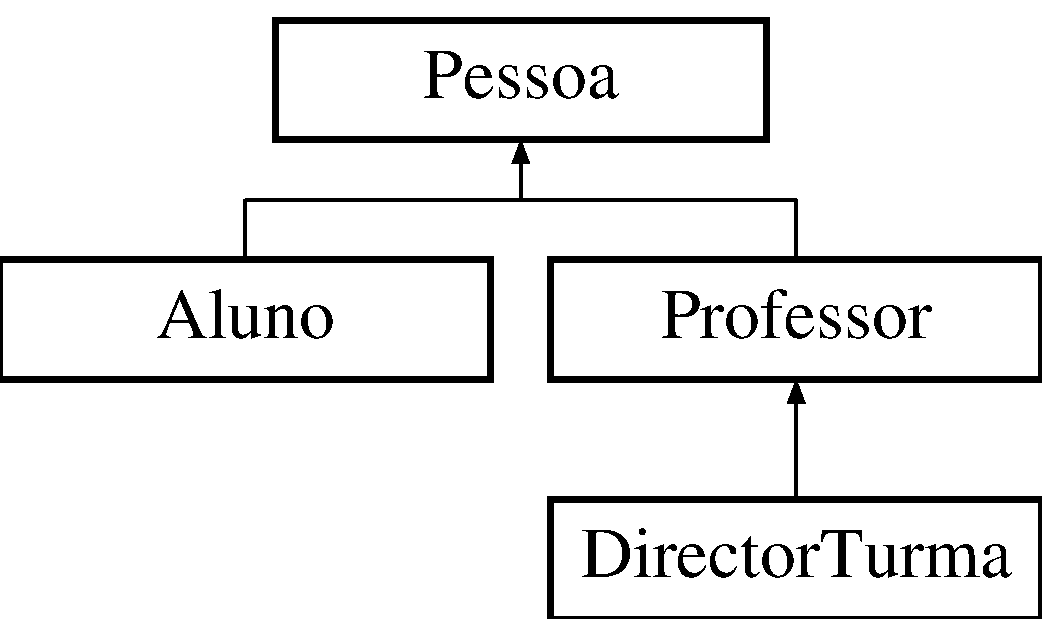
\includegraphics[height=3.000000cm]{class_pessoa}
\end{center}
\end{figure}
\subsection*{Public Member Functions}
\begin{DoxyCompactItemize}
\item 
\hypertarget{class_pessoa_a789675384a5b47a16c9f0a5a819aa1ff}{{\bfseries Pessoa} (string n)}\label{class_pessoa_a789675384a5b47a16c9f0a5a819aa1ff}

\item 
\hypertarget{class_pessoa_afe5128d96f8ef52b644746b9a45f63e7}{void {\bfseries set\-Nome} (const string n)}\label{class_pessoa_afe5128d96f8ef52b644746b9a45f63e7}

\item 
\hypertarget{class_pessoa_a8d4d2f40ba5634f49b0ce181fee7f0a7}{string {\bfseries get\-Nome} () const }\label{class_pessoa_a8d4d2f40ba5634f49b0ce181fee7f0a7}

\item 
\hypertarget{class_pessoa_a6ccbd5e11c47beb6de6650054caa5a79}{virtual string {\bfseries print} ()}\label{class_pessoa_a6ccbd5e11c47beb6de6650054caa5a79}

\end{DoxyCompactItemize}


\subsection{Detailed Description}
Classe Base para \hyperlink{class_professor}{Professor} e \hyperlink{class_aluno}{Aluno}. 

The documentation for this class was generated from the following file\-:\begin{DoxyCompactItemize}
\item 
Professor.\-h\end{DoxyCompactItemize}

\hypertarget{class_professor}{\section{Professor Class Reference}
\label{class_professor}\index{Professor@{Professor}}
}


\hyperlink{class_professor}{Professor} de uma \hyperlink{class_escola}{Escola} (class Base), podendo ou nao ser Director de \hyperlink{class_turma}{Turma}.  




{\ttfamily \#include $<$Professor.\-h$>$}

Inheritance diagram for Professor\-:\begin{figure}[H]
\begin{center}
\leavevmode
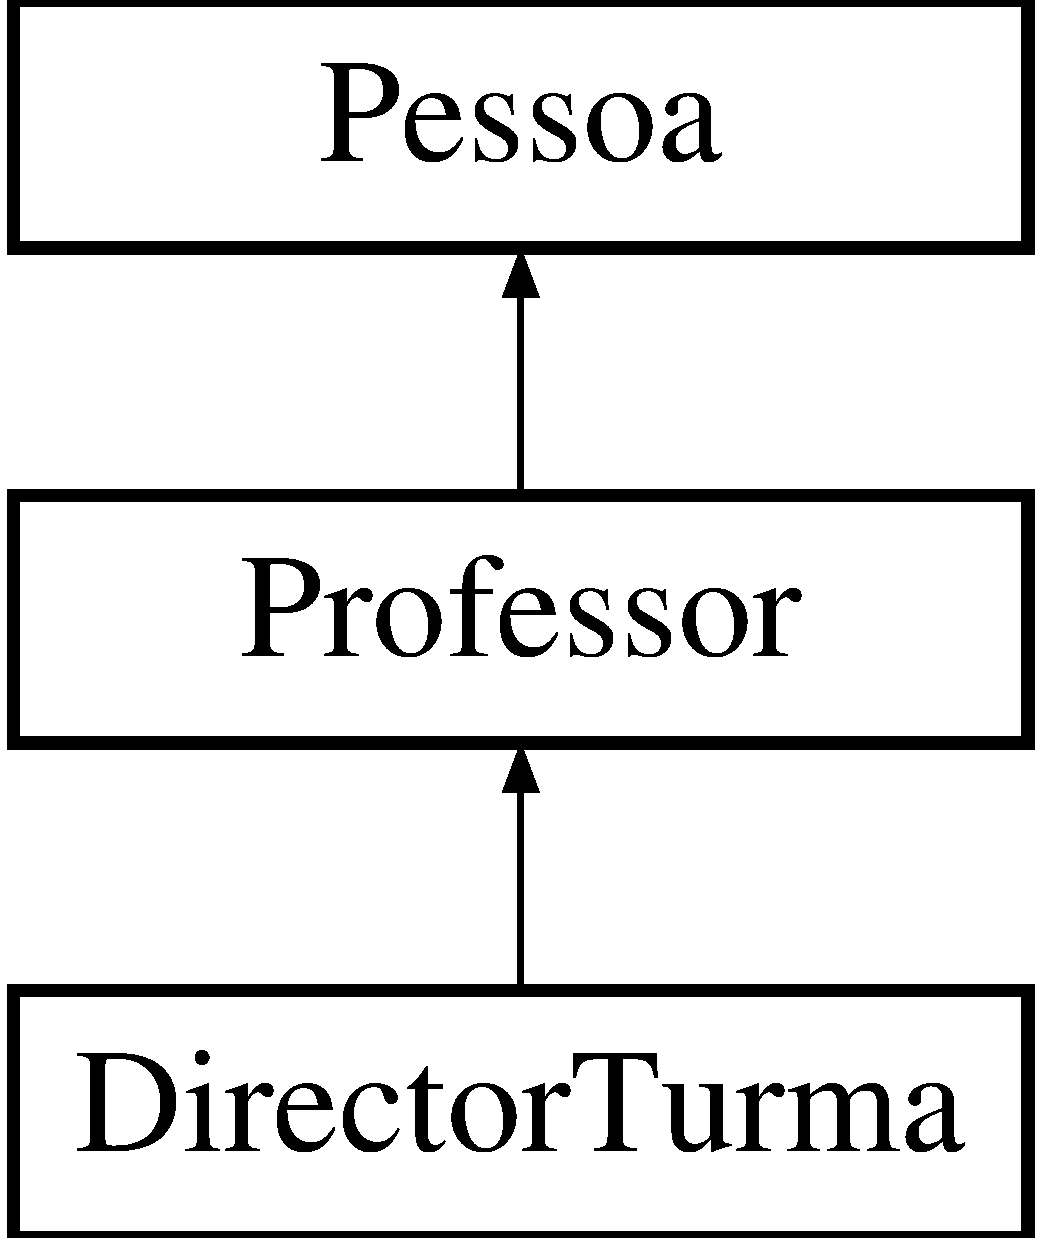
\includegraphics[height=3.000000cm]{class_professor}
\end{center}
\end{figure}
\subsection*{Public Member Functions}
\begin{DoxyCompactItemize}
\item 
\hypertarget{class_professor_a8e20e8472f95da9e7dbbe043b2ca40c0}{\hyperlink{class_professor_a8e20e8472f95da9e7dbbe043b2ca40c0}{Professor} (string n, \hyperlink{class_disciplina}{Disciplina} $\ast$d, \hyperlink{class_turma}{Turma} $\ast$t)}\label{class_professor_a8e20e8472f95da9e7dbbe043b2ca40c0}

\begin{DoxyCompactList}\small\item\em Construtor de \hyperlink{class_professor}{Professor} inicializando com o minimo de uma turma. \end{DoxyCompactList}\item 
\hypertarget{class_professor_a4242c678534b7effaec214ad2f8a3079}{bool \hyperlink{class_professor_a4242c678534b7effaec214ad2f8a3079}{add\-Turma} (\hyperlink{class_turma}{Turma} $\ast$t)}\label{class_professor_a4242c678534b7effaec214ad2f8a3079}

\begin{DoxyCompactList}\small\item\em Adiciona uma \hyperlink{class_turma}{Turma} as do \hyperlink{class_professor}{Professor}. \end{DoxyCompactList}\item 
\hypertarget{class_professor_a1cc34746e255348252f50e0b6ab34e41}{bool \hyperlink{class_professor_a1cc34746e255348252f50e0b6ab34e41}{remove\-Turma} (const int id)}\label{class_professor_a1cc34746e255348252f50e0b6ab34e41}

\begin{DoxyCompactList}\small\item\em Remove uma \hyperlink{class_turma}{Turma} das do \hyperlink{class_professor}{Professor}. \end{DoxyCompactList}\item 
\hypertarget{class_professor_a3fcf6e5e91713f69e178d3c77524f9bc}{string {\bfseries print} ()}\label{class_professor_a3fcf6e5e91713f69e178d3c77524f9bc}

\item 
\hypertarget{class_professor_a6670967a09f78b6d0016a2e3417c238f}{void {\bfseries set\-Disciplina} (\hyperlink{class_disciplina}{Disciplina} $\ast$d)}\label{class_professor_a6670967a09f78b6d0016a2e3417c238f}

\item 
\hypertarget{class_professor_ae09b97fead0e86fa47e9d477a1f4b1d5}{\hyperlink{class_disciplina}{Disciplina} $\ast$ {\bfseries get\-Discipina} () const }\label{class_professor_ae09b97fead0e86fa47e9d477a1f4b1d5}

\item 
\hypertarget{class_professor_a9474309b22807309eacd155312b9f65d}{vector$<$ \hyperlink{class_turma}{Turma} $\ast$ $>$ {\bfseries get\-Turmas} () const }\label{class_professor_a9474309b22807309eacd155312b9f65d}

\item 
\hypertarget{class_professor_afa33df5062ac3fd56de2a54530bd1c68}{bool {\bfseries operator==} (\hyperlink{class_professor}{Professor} $\ast$p2)}\label{class_professor_afa33df5062ac3fd56de2a54530bd1c68}

\end{DoxyCompactItemize}


\subsection{Detailed Description}
\hyperlink{class_professor}{Professor} de uma \hyperlink{class_escola}{Escola} (class Base), podendo ou nao ser Director de \hyperlink{class_turma}{Turma}. 

The documentation for this class was generated from the following files\-:\begin{DoxyCompactItemize}
\item 
Professor.\-h\item 
Professor.\-cpp\end{DoxyCompactItemize}

\hypertarget{class_professor_nao_existente}{\section{Professor\-Nao\-Existente Class Reference}
\label{class_professor_nao_existente}\index{Professor\-Nao\-Existente@{Professor\-Nao\-Existente}}
}


Excepcao lancada quando o \hyperlink{class_professor}{Professor} a ser acedido nao existe.  




{\ttfamily \#include $<$Excepcao.\-h$>$}

\subsection*{Public Member Functions}
\begin{DoxyCompactItemize}
\item 
\hypertarget{class_professor_nao_existente_a010426aacae28cf35fd7b82d51a92c92}{{\bfseries Professor\-Nao\-Existente} (\hyperlink{class_professor}{Professor} $\ast$p)}\label{class_professor_nao_existente_a010426aacae28cf35fd7b82d51a92c92}

\item 
string \hyperlink{class_professor_nao_existente_a7e4f7530740f578c181f1e8d05404104}{get\-Erro} ()
\item 
\hypertarget{class_professor_nao_existente_ad0582a609813717d969ba09d93b7c1ff}{virtual \hyperlink{class_professor_nao_existente_ad0582a609813717d969ba09d93b7c1ff}{$\sim$\-Professor\-Nao\-Existente} ()}\label{class_professor_nao_existente_ad0582a609813717d969ba09d93b7c1ff}

\begin{DoxyCompactList}\small\item\em Destrutor. \end{DoxyCompactList}\end{DoxyCompactItemize}
\subsection*{Public Attributes}
\begin{DoxyCompactItemize}
\item 
\hypertarget{class_professor_nao_existente_ac9d47ada01b74d050825da7e7517bf2e}{\hyperlink{class_professor}{Professor} $\ast$ \hyperlink{class_professor_nao_existente_ac9d47ada01b74d050825da7e7517bf2e}{professor}}\label{class_professor_nao_existente_ac9d47ada01b74d050825da7e7517bf2e}

\begin{DoxyCompactList}\small\item\em \hyperlink{class_aluno}{Aluno} inesxistente. \end{DoxyCompactList}\end{DoxyCompactItemize}


\subsection{Detailed Description}
Excepcao lancada quando o \hyperlink{class_professor}{Professor} a ser acedido nao existe. 

\subsection{Member Function Documentation}
\hypertarget{class_professor_nao_existente_a7e4f7530740f578c181f1e8d05404104}{\index{Professor\-Nao\-Existente@{Professor\-Nao\-Existente}!get\-Erro@{get\-Erro}}
\index{get\-Erro@{get\-Erro}!ProfessorNaoExistente@{Professor\-Nao\-Existente}}
\subsubsection[{get\-Erro}]{\setlength{\rightskip}{0pt plus 5cm}string Professor\-Nao\-Existente\-::get\-Erro (
\begin{DoxyParamCaption}
{}
\end{DoxyParamCaption}
)\hspace{0.3cm}{\ttfamily [inline]}}}\label{class_professor_nao_existente_a7e4f7530740f578c181f1e8d05404104}
$<$ Mensagem de erro lancada pela excepcao 

The documentation for this class was generated from the following file\-:\begin{DoxyCompactItemize}
\item 
Excepcao.\-h\end{DoxyCompactItemize}

\hypertarget{class_turma}{\section{Turma Class Reference}
\label{class_turma}\index{Turma@{Turma}}
}
\subsection*{Public Member Functions}
\begin{DoxyCompactItemize}
\item 
\hypertarget{class_turma_a8ad1feec07b4c0ff5d4ec51c8b4a61fd}{\hyperlink{class_turma_a8ad1feec07b4c0ff5d4ec51c8b4a61fd}{Turma} ()}\label{class_turma_a8ad1feec07b4c0ff5d4ec51c8b4a61fd}

\begin{DoxyCompactList}\small\item\em default empty constructor for \hyperlink{class_turma}{Turma} \end{DoxyCompactList}\item 
\hyperlink{class_turma_a6a392c8d9e5b824ce0460740c9bfcdc9}{Turma} (int id, int ano\-Escolar)
\begin{DoxyCompactList}\small\item\em Constructor non-\/empty for \hyperlink{class_turma}{Turma}. \end{DoxyCompactList}\item 
\hyperlink{class_turma_a68d82f9338997281af20221fff43b509}{Turma} (int id)
\item 
\hypertarget{class_turma_ac9901558278461593150226ed06567e2}{virtual \hyperlink{class_turma_ac9901558278461593150226ed06567e2}{$\sim$\-Turma} ()}\label{class_turma_ac9901558278461593150226ed06567e2}

\begin{DoxyCompactList}\small\item\em Default destructor. \end{DoxyCompactList}\item 
int \hyperlink{class_turma_a25bc31537a7fb3345712b780ff2f825f}{get\-I\-D} ()
\item 
int \hyperlink{class_turma_a18af6d19b01102c00f07720f7b149252}{get\-Ano\-Escolar} ()
\item 
\hyperlink{class_horario}{Horario} $\ast$ \hyperlink{class_turma_af23a78e8b0130542d662f9d1c20b9422}{get\-Horario} ()
\item 
void \hyperlink{class_turma_a5c011a25251cd40d549e504b71d7b18f}{set\-I\-D} (int i)
\item 
void \hyperlink{class_turma_abd1be35d1d394aeca1818ed643845ff8}{set\-Ano\-Escolar} (int ae)
\item 
void \hyperlink{class_turma_aab28fe642d927ba176ec4259fdc2d8e0}{set\-Horario} (\hyperlink{class_horario}{Horario} $\ast$h)
\item 
bool \hyperlink{class_turma_a52d07a750b962cfb81c2067858d9d08a}{operator==} (\hyperlink{class_turma}{Turma} $\ast$t2)
\end{DoxyCompactItemize}


\subsection{Constructor \& Destructor Documentation}
\hypertarget{class_turma_a6a392c8d9e5b824ce0460740c9bfcdc9}{\index{Turma@{Turma}!Turma@{Turma}}
\index{Turma@{Turma}!Turma@{Turma}}
\subsubsection[{Turma}]{\setlength{\rightskip}{0pt plus 5cm}Turma\-::\-Turma (
\begin{DoxyParamCaption}
\item[{int}]{id, }
\item[{int}]{ano\-Escolar}
\end{DoxyParamCaption}
)}}\label{class_turma_a6a392c8d9e5b824ce0460740c9bfcdc9}


Constructor non-\/empty for \hyperlink{class_turma}{Turma}. 


\begin{DoxyParams}{Parameters}
{\em id} & \\
\hline
{\em ano\-Escolar} & \\
\hline
\end{DoxyParams}
\hypertarget{class_turma_a68d82f9338997281af20221fff43b509}{\index{Turma@{Turma}!Turma@{Turma}}
\index{Turma@{Turma}!Turma@{Turma}}
\subsubsection[{Turma}]{\setlength{\rightskip}{0pt plus 5cm}Turma\-::\-Turma (
\begin{DoxyParamCaption}
\item[{int}]{id}
\end{DoxyParamCaption}
)}}\label{class_turma_a68d82f9338997281af20221fff43b509}

\begin{DoxyParams}{Parameters}
{\em id} & \\
\hline
\end{DoxyParams}


\subsection{Member Function Documentation}
\hypertarget{class_turma_a18af6d19b01102c00f07720f7b149252}{\index{Turma@{Turma}!get\-Ano\-Escolar@{get\-Ano\-Escolar}}
\index{get\-Ano\-Escolar@{get\-Ano\-Escolar}!Turma@{Turma}}
\subsubsection[{get\-Ano\-Escolar}]{\setlength{\rightskip}{0pt plus 5cm}int Turma\-::get\-Ano\-Escolar (
\begin{DoxyParamCaption}
{}
\end{DoxyParamCaption}
)}}\label{class_turma_a18af6d19b01102c00f07720f7b149252}
\begin{DoxyReturn}{Returns}

\end{DoxyReturn}
\hypertarget{class_turma_af23a78e8b0130542d662f9d1c20b9422}{\index{Turma@{Turma}!get\-Horario@{get\-Horario}}
\index{get\-Horario@{get\-Horario}!Turma@{Turma}}
\subsubsection[{get\-Horario}]{\setlength{\rightskip}{0pt plus 5cm}{\bf Horario} $\ast$ Turma\-::get\-Horario (
\begin{DoxyParamCaption}
{}
\end{DoxyParamCaption}
)}}\label{class_turma_af23a78e8b0130542d662f9d1c20b9422}
\begin{DoxyReturn}{Returns}

\end{DoxyReturn}
\hypertarget{class_turma_a25bc31537a7fb3345712b780ff2f825f}{\index{Turma@{Turma}!get\-I\-D@{get\-I\-D}}
\index{get\-I\-D@{get\-I\-D}!Turma@{Turma}}
\subsubsection[{get\-I\-D}]{\setlength{\rightskip}{0pt plus 5cm}int Turma\-::get\-I\-D (
\begin{DoxyParamCaption}
{}
\end{DoxyParamCaption}
)}}\label{class_turma_a25bc31537a7fb3345712b780ff2f825f}
\begin{DoxyReturn}{Returns}

\end{DoxyReturn}
\hypertarget{class_turma_a52d07a750b962cfb81c2067858d9d08a}{\index{Turma@{Turma}!operator==@{operator==}}
\index{operator==@{operator==}!Turma@{Turma}}
\subsubsection[{operator==}]{\setlength{\rightskip}{0pt plus 5cm}bool Turma\-::operator== (
\begin{DoxyParamCaption}
\item[{{\bf Turma} $\ast$}]{t2}
\end{DoxyParamCaption}
)}}\label{class_turma_a52d07a750b962cfb81c2067858d9d08a}

\begin{DoxyParams}{Parameters}
{\em t2} & \\
\hline
\end{DoxyParams}
\begin{DoxyReturn}{Returns}

\end{DoxyReturn}
\hypertarget{class_turma_abd1be35d1d394aeca1818ed643845ff8}{\index{Turma@{Turma}!set\-Ano\-Escolar@{set\-Ano\-Escolar}}
\index{set\-Ano\-Escolar@{set\-Ano\-Escolar}!Turma@{Turma}}
\subsubsection[{set\-Ano\-Escolar}]{\setlength{\rightskip}{0pt plus 5cm}void Turma\-::set\-Ano\-Escolar (
\begin{DoxyParamCaption}
\item[{int}]{ae}
\end{DoxyParamCaption}
)}}\label{class_turma_abd1be35d1d394aeca1818ed643845ff8}

\begin{DoxyParams}{Parameters}
{\em ae} & \\
\hline
\end{DoxyParams}
\hypertarget{class_turma_aab28fe642d927ba176ec4259fdc2d8e0}{\index{Turma@{Turma}!set\-Horario@{set\-Horario}}
\index{set\-Horario@{set\-Horario}!Turma@{Turma}}
\subsubsection[{set\-Horario}]{\setlength{\rightskip}{0pt plus 5cm}void Turma\-::set\-Horario (
\begin{DoxyParamCaption}
\item[{{\bf Horario} $\ast$}]{h}
\end{DoxyParamCaption}
)}}\label{class_turma_aab28fe642d927ba176ec4259fdc2d8e0}

\begin{DoxyParams}{Parameters}
{\em h} & \\
\hline
\end{DoxyParams}
\hypertarget{class_turma_a5c011a25251cd40d549e504b71d7b18f}{\index{Turma@{Turma}!set\-I\-D@{set\-I\-D}}
\index{set\-I\-D@{set\-I\-D}!Turma@{Turma}}
\subsubsection[{set\-I\-D}]{\setlength{\rightskip}{0pt plus 5cm}void Turma\-::set\-I\-D (
\begin{DoxyParamCaption}
\item[{int}]{i}
\end{DoxyParamCaption}
)}}\label{class_turma_a5c011a25251cd40d549e504b71d7b18f}

\begin{DoxyParams}{Parameters}
{\em i} & \\
\hline
\end{DoxyParams}


The documentation for this class was generated from the following files\-:\begin{DoxyCompactItemize}
\item 
Turma.\-h\item 
Turma.\-cpp\end{DoxyCompactItemize}

\hypertarget{class_turma_existente}{\section{Turma\-Existente Class Reference}
\label{class_turma_existente}\index{Turma\-Existente@{Turma\-Existente}}
}


Excepcao lancada quando uma \hyperlink{class_turma}{Turma} a ser adicionada ao vector de Turmas de uma \hyperlink{class_professor}{Professor} que ja contem a mesma.  




{\ttfamily \#include $<$Excepcao.\-h$>$}

\subsection*{Public Member Functions}
\begin{DoxyCompactItemize}
\item 
\hypertarget{class_turma_existente_abc57fc0e6dc6b40e7e09a55dc572aea9}{{\bfseries Turma\-Existente} (\hyperlink{class_turma}{Turma} $\ast$t)}\label{class_turma_existente_abc57fc0e6dc6b40e7e09a55dc572aea9}

\item 
string \hyperlink{class_turma_existente_a96340570dfd3b2a4122c8ba8820dac4a}{get\-Erro} ()
\item 
\hypertarget{class_turma_existente_a6b3ec0715645fd0ea2589dace1ccd0bf}{virtual \hyperlink{class_turma_existente_a6b3ec0715645fd0ea2589dace1ccd0bf}{$\sim$\-Turma\-Existente} ()}\label{class_turma_existente_a6b3ec0715645fd0ea2589dace1ccd0bf}

\begin{DoxyCompactList}\small\item\em Destrutor. \end{DoxyCompactList}\end{DoxyCompactItemize}
\subsection*{Public Attributes}
\begin{DoxyCompactItemize}
\item 
\hypertarget{class_turma_existente_a7af4e8a63dd324498ebd01cee1a956f3}{\hyperlink{class_turma}{Turma} $\ast$ \hyperlink{class_turma_existente_a7af4e8a63dd324498ebd01cee1a956f3}{turma}}\label{class_turma_existente_a7af4e8a63dd324498ebd01cee1a956f3}

\begin{DoxyCompactList}\small\item\em \hyperlink{class_turma}{Turma} ja existente. \end{DoxyCompactList}\end{DoxyCompactItemize}


\subsection{Detailed Description}
Excepcao lancada quando uma \hyperlink{class_turma}{Turma} a ser adicionada ao vector de Turmas de uma \hyperlink{class_professor}{Professor} que ja contem a mesma. 

\subsection{Member Function Documentation}
\hypertarget{class_turma_existente_a96340570dfd3b2a4122c8ba8820dac4a}{\index{Turma\-Existente@{Turma\-Existente}!get\-Erro@{get\-Erro}}
\index{get\-Erro@{get\-Erro}!TurmaExistente@{Turma\-Existente}}
\subsubsection[{get\-Erro}]{\setlength{\rightskip}{0pt plus 5cm}string Turma\-Existente\-::get\-Erro (
\begin{DoxyParamCaption}
{}
\end{DoxyParamCaption}
)\hspace{0.3cm}{\ttfamily [inline]}}}\label{class_turma_existente_a96340570dfd3b2a4122c8ba8820dac4a}
$<$ Mensagem de erro lancada por esta excepcao 

The documentation for this class was generated from the following file\-:\begin{DoxyCompactItemize}
\item 
Excepcao.\-h\end{DoxyCompactItemize}

\hypertarget{class_turma_nao_existente}{\section{Turma\-Nao\-Existente Class Reference}
\label{class_turma_nao_existente}\index{Turma\-Nao\-Existente@{Turma\-Nao\-Existente}}
}


Excepcao lancada quando a \hyperlink{class_turma}{Turma} a ser acedida nao existe.  




{\ttfamily \#include $<$Excepcao.\-h$>$}

\subsection*{Public Member Functions}
\begin{DoxyCompactItemize}
\item 
\hypertarget{class_turma_nao_existente_a9c2b3b2ad6de696dd3432951b278c975}{{\bfseries Turma\-Nao\-Existente} (\hyperlink{class_turma}{Turma} $\ast$t)}\label{class_turma_nao_existente_a9c2b3b2ad6de696dd3432951b278c975}

\item 
string \hyperlink{class_turma_nao_existente_a5672fe80509c285ce4468137c3574351}{get\-Erro} ()
\item 
\hypertarget{class_turma_nao_existente_a89025d5c39ff6a1590e2e7bb010fa3b7}{virtual \hyperlink{class_turma_nao_existente_a89025d5c39ff6a1590e2e7bb010fa3b7}{$\sim$\-Turma\-Nao\-Existente} ()}\label{class_turma_nao_existente_a89025d5c39ff6a1590e2e7bb010fa3b7}

\begin{DoxyCompactList}\small\item\em Destrutor. \end{DoxyCompactList}\end{DoxyCompactItemize}
\subsection*{Public Attributes}
\begin{DoxyCompactItemize}
\item 
\hypertarget{class_turma_nao_existente_ab14dc459c3d9bd70bea8e583b2ce072e}{\hyperlink{class_turma}{Turma} $\ast$ \hyperlink{class_turma_nao_existente_ab14dc459c3d9bd70bea8e583b2ce072e}{turma}}\label{class_turma_nao_existente_ab14dc459c3d9bd70bea8e583b2ce072e}

\begin{DoxyCompactList}\small\item\em \hyperlink{class_turma}{Turma} inesxistente. \end{DoxyCompactList}\end{DoxyCompactItemize}


\subsection{Detailed Description}
Excepcao lancada quando a \hyperlink{class_turma}{Turma} a ser acedida nao existe. 

\subsection{Member Function Documentation}
\hypertarget{class_turma_nao_existente_a5672fe80509c285ce4468137c3574351}{\index{Turma\-Nao\-Existente@{Turma\-Nao\-Existente}!get\-Erro@{get\-Erro}}
\index{get\-Erro@{get\-Erro}!TurmaNaoExistente@{Turma\-Nao\-Existente}}
\subsubsection[{get\-Erro}]{\setlength{\rightskip}{0pt plus 5cm}string Turma\-Nao\-Existente\-::get\-Erro (
\begin{DoxyParamCaption}
{}
\end{DoxyParamCaption}
)\hspace{0.3cm}{\ttfamily [inline]}}}\label{class_turma_nao_existente_a5672fe80509c285ce4468137c3574351}
$<$ Mensagem de erro lancada pela excepcao 

The documentation for this class was generated from the following file\-:\begin{DoxyCompactItemize}
\item 
Excepcao.\-h\end{DoxyCompactItemize}

\addcontentsline{toc}{part}{Index}
\printindex
\end{document}
